\documentclass[a4paper,12pt,twoside,openany]{report}

\usepackage{polski}
\usepackage{helvet}
\usepackage[T1]{fontenc}
\usepackage{anyfontsize}
\usepackage[utf8]{inputenc}
\usepackage[pdftex]{graphicx}
\usepackage{tabularx}
\usepackage{array}
\usepackage[polish]{babel}
\usepackage{subfigure}
\usepackage{amsfonts}
\usepackage{verbatim}
\usepackage{indentfirst}
\usepackage[pdftex]{hyperref}


\newcommand{\rys}{.}

% oznaczenie rzeczy do zrobienia/poprawienia
\newcommand{\TODO}{\textbf{TODO}}


% wyroznienie slow kluczowych
\newcommand{\tech}{\texttt}

% na oprawe (1.0cm - 0.7cm)*2 = 0.6cm
% na oprawe (1.1cm - 0.7cm)*2 = 0.8cm
%  oddsidemargin lewy margines na nieparzystych stronach
% evensidemargin lewy margines na parzystych stronach
\def\oprawa{1.05cm}
\addtolength{\oddsidemargin}{\oprawa}
\addtolength{\evensidemargin}{-\oprawa}

% table span multirows
\usepackage{multirow}
\usepackage{enumitem}	% enumitem.pdf
\setlist{listparindent=\parindent, parsep=\parskip} % potrzebuje enumitem

%%%%%%%%%%%%%%% Dodatkowe Pakiety %%%%%%%%%%%%%%%%%
\usepackage{prmag2017}   % definiuje komendy opieku,nrindeksu, rodzaj pracy, ...


%%%%%%%%%%%%%%% Strona Tytułowa %%%%%%%%%%%%%%%%%
% To trzeba wypelnic swoimi danymi
\title{Porównanie progresywnych aplikacji internetowych i aplikacji hybrydowych}

% autor
\author{Marta Wi\'sniewska}
\nrindeksu{252217}

\opiekun{prof. nzw. dr hab. inż. Krzysztof Siwek}
\terminwykonania{1 czerwca 2018} % data na oświadczeniu o samodzielności
\rok{2018}


% To sa domyslne wartosci
% - mozna je zmienic, jesli praca jest pisana gdzie indziej niz w ZETiIS
% - mozna je wyrzucic jesli praca jest pisana w ZETiIS
%\miasto{Warszawa}
%\uczelnia{POLITECHNIKA WARSZAWSKA}
%\wydzial{WYDZIAŁ ELEKTRYCZNY}
%\instytut{INSTYTUT ELEKTROTECHNIKI TEORETYCZNEJ\linebreak[1] I~SYSTEMÓW INFORMACYJNO-POMIAROWYCH}
% \zaklad{ZAKŁAD ELEKTROTECHNIKI TEORETYCZNEJ\linebreak[1] I~INFORMATYKI STOSOWANEJ}
%\kierunekstudiow{INFORMATYKA}

% domyslnie praca jest inzynierska, ale po odkomentowaniu ponizszej linii zrobi sie magisterska
\pracamagisterska
%%% koniec od P.W

\opinie{%
  \newpage
\begin{center}
 {\large\bf  Opinia} \\
o pracy dyplomowej magisterskiej wykonanej przez dyplomanta\\
{\bf Zdolnego Studenta i Pracowitego Kolegę} \\
 Wydział Elektryczny, kierunek Informatyka,  Politechnika Warszawska\\
Temat pracy\\
\textit{\bf
TYTUŁ PRACY DYPLOMOWEJ
}\\
\end{center}
\medskip
\noindent
Promotor: {\bf dr inż. Miły Opiekun}\\
Ocena pracy dyplomowej: {\bf bardzo dobry}

\medskip

\centerline{\bf Treść opinii}
   Celem pracy dyplomowej panów dolnego Studenta i Pracowitego Kolegi  było
opracowanie systemu pozwalającego symulować  i opartego o oprogramowanie o
otwartych źródłach (ang. Open Source). Jak piszą Dyplomanci, starali się opracować
system, który łatwo będzie dostosować do zmieniających się dynamicznie wymagań,
będzie miał niewielkie wymagania sprzętowe i umożliwiał dalszą łatwą rozbudowę oraz
dostosowanie go do potrzeb.
Przedstawiona do recenzji praca składa się z krótkiego wstępu jasno i
wyczerpująco opisującego oraz uzasadniającego cel pracy, trzech rozdziałów (2-4)
zawierających opis istniejących podobnych
rozwiązań, komponentów rozpatrywanychjako kandydaci do
tworzonego systemu i wreszcie zagadnień wydajności wirtualnych
rozwiązań. Piąty rozdział to opis przygotowanego przez
Dyplomantów środowiska obejmujący opis konfiguracji
środowiska oraz przykładowe ćwiczenia laboratoryjne. Ostatni
rozdział pracy to opis możliwości dalszego
rozwoju projektu. W ramach przygotowania pracy Dyplomanci zebrali i przedstawili w
bardzo przejrzysty sposób duży zasób informacji, co świadczy o dobrej orientacji
w nowoczesnej i ciągle intensywnie rozwijanej tematyce stanowiącej
zakres pracy i o umiejętności przejrzystego przedstawienia tych
wyników. Praca zawiera dwa dodatki, z których pierwszy obejmuje wyniki
eksperymentów i badań nad wydajnością, a drugi to źródła
skryptów budujących środowisko.

 Dyplomanci dość
dobrze zrealizowali postawione przed nimi zadanie,
wykazali się więc umiejętnością zastosowania w praktyce wiedzy
przedstawionej w rozdziałach 2-4.  Uważam, że cele postawione w założeniach pracy zostały pomyślnie
zrealizowane. Proponuję ocenę bardzo dobrą (5).

\vskip 1cm
{
\raggedleft
(data, podpis)\kern1cm

}
  \newpage
  \newpage
\begin{center}
 {\large\bf  Recenzja } \\
pracy dyplomowej magisterskiej wykonanej przez dyplomanta\\
{\bf Zdolnego Studenta i Pracowitego Kolegę} \\
 Wydział Elektryczny, kierunek Informatyka,  Politechnika Warszawska\\
Temat pracy\\
\textit{\bf
TYTUŁ PRACY DYPLOMOWEJ
}\\
\end{center}
\medskip
\noindent
Recenzent: {\bf prof. nzw. dr hab. inż. Jan Surowy}\\
Ocena pracy dyplomowej: {\bf bardzo dobry}
\medskip


\centerline{\bf Treść recenzji}
   Celem pracy dyplomowej panów dolnego Studenta i Pracowitego Kolegi  było
opracowanie systemu pozwalającego symulować  i opartego o oprogramowanie o
otwartych źródłach (ang. Open Source). Jak piszą Dyplomanci, starali się opracować
system, który łatwo będzie dostosować do zmieniających się dynamicznie wymagań,
będzie miał niewielkie wymagania sprzętowe i umożliwiał dalszą łatwą rozbudowę oraz
dostosowanie go do potrzeb.
Przedstawiona do recenzji praca składa się z krótkiego wstępu jasno i
wyczerpująco opisującego oraz uzasadniającego cel pracy, trzech rozdziałów (2-4)
zawierających bardzo solidny i przejrzysty opis: istniejących podobnych
rozwiązań (rozdz. 2), komponentów rozpatrywanychjako kandydaci do
tworzonego systemu (rozdz. 3) i wreszcie zagadnień wydajności wirtualnych
rozwiązań, zwłaszcza w kontekście współpracy  kilku elementów
 sieci (rozdział 4). Piąty rozdział to opis przygotowanego przez
Dyplomantów środowiska obejmujący opis konfiguracji
środowiska oraz przykładowe ćwiczenia laboratoryjne (5 ćwiczeń). Ostatni, szósty
rozdział pracy to krótkie zakończenie, które wylicza także możliwości dalszego
rozwoju projektu. W ramach przygotowania pracy Dyplomanci zebrali i przedstawili w
bardzo przejrzysty sposób duży zasób informacji o narzędziach, Rozdziały 2, 3 i 4 świadczą o dobrej orientacji
w nowoczesnej i ciągle intensywnie rozwijanej tematyce stanowiącej
zakres pracy i o umiejętności syntetycznego, przejrzystego przedstawienia tych
wyników. Drobne  mankamenty tej części pracy to zbyt skrótowe omawianie
niektórych zagadnień technicznych, zakładające dużą początkową wiedzę czytelnika
i dość niestaranne podejście do powołań na źródła.
Utrudnia to w pewnym stopniu czytanie pracy i zmniejsza jej wartość dydaktyczną
(a ta zdaje się być jednym z celów Autorów), ale jest zrekompensowane zawartością
merytoryczną. Praca zawiera dwa dodatki, z których pierwszy obejmuje wyniki
eksperymentów i badań nad wydajnością, a drugi to źródła
skryptów budujących środowisko. Praca
zawiera niestety dość dużą liczbę drobnych błędów redakcyjnych, ale nie wpływają
one w sposób istotny na na jej czytelność i wartość. W całej pracy przewijają
się samodzielne, zdecydowane wnioski Autorów, które są wynikiem własnych i
oryginalnych badań.  Rozdział 5 i dodatki pracy przekonują mnie, że Dyplomanci dość
dobrze zrealizowali postawione przed nimi zadanie. Pozwala to stwierdzić, że
wykazali się więc także umiejętnością zastosowania w praktyce wiedzy
przedstawionej w rozdziałach 2-4. Kończący pracę rozdział szósty świadczy o
dużym (ale moim zdaniem uzasadnionym) poczuciu własnej wartości i jest
świadectwem własnego, oryginalnego spojrzenia na tematykę przedstawioną w pracy
dyplomowej. Uważam, że cele postawione w założeniach pracy zostały pomyślnie
zrealizowane. Proponuję ocenę bardzo dobrą (5).

\vskip 1cm
{
\raggedleft
(data, podpis)\kern1cm

}
}

\streszczenia{
  \newpage
\begin{center}
\large \bf
PORÓWNANIE PROGRESYWNYCH APLIKACJI INTERNETOWYCH I APLIKACJI HYBRYDOWYCH
\end{center}

\section*{Streszczenie}
Praca składa się z krótkiego wstępu jasno i
wyczerpująco opisującego oraz uzasadniającego cel pracy, trzech rozdziałów (2-4)
zawierających opis istniejących podobnych
rozwiązań, komponentów rozpatrywanychjako kandydaci do
tworzonego systemu i wreszcie zagadnień wydajności wirtualnych
rozwiązań. Piąty rozdział to opis  środowiska obejmujący opis konfiguracji
środowiska oraz przykładowe ćwiczenia laboratoryjne. Ostatni
rozdział pracy to opis możliwości dalszego
rozwoju projektu. 

\bigskip
{\noindent\bf Słowa kluczowe:} progresywne aplikacje internetowe, aplikacje hybrydowe, aplikacje natywne

\vskip 2cm


\begin{center}
\large \bf
THESIS TITLE
\end{center}

\section*{Abstract}
This thesis presents a novel way of using a novel algorithm to solve complex
problems of filter design. In the first chapter the fundamentals of filter design
are presented. The second chapter describes an original algorithm invented by the
authors. Is is based on evolution strategy, but uses an original method of filter
description similar to artificial neural network. In the third chapter the implementation
of the algorithm in C programming language is presented. The fifth chapter contains results
of tests which prove high efficiency and enormous accuracy of the program. Finally some
posibilities of further development of the invented algoriths are proposed.

\bigskip
{\noindent\bf Keywords:} progressive web apps, hybrid apps, native apps

\vfill
}

\begin{document}
\maketitle

%-----------------
% Wstęp
%-----------------
\chapter{Wstęp}
Użytkownicy spędzają coraz więcej czasu na urządzeniach mobilnych, więc zadbanie o to, aby witryny mobilne spełniały ich oczekiwania, jest niezwykle ważne. Z jednej strony jeśli witryna Twojego klienta ładuje się zbyt wolno, użytkownicy zrezygnują z korzystania z niej. Z drugiej strony szybko ładująca się, ale źle zaprojektowana witryna utrudnia użytkownikom wykonanie pożądanych działań. W świecie, gdzie urządzenia mobilne są coraz bardziej powszechne, oczekiwania konsumentów są wysokie. W tym module dowiesz się, dlaczego wygoda użytkowników i szybkość witryn mobilnych są ważne.



%-----------------
% Aplikacje mobilne
%-----------------
\chapter {Aplikacje mobilne}
Urządzenia mobilne na przestrzeni ostanich kilku lat zdobyły ogromną popularno\'sć. Ma to duży wpływ na rozwój aplikacji internetowych i możliwo\'sci ich wykorzystania na różnych urządzeniach mobilnych. Użytkownicy aplikacji sieciowych coraz czę\'sciej używają urządzeń mobilnych, rezygnując z korzystania z przeglądarki komputera. Na wykresie \ref{fig:plot1} zaprezentowano jak na przestrzeni lat 2015-2018 zmieniał się udział odsłon aplikacji sieciowych z różnych platform - komputera, telefonu, tabletu. 
\begin{figure}[h]
    \centering
    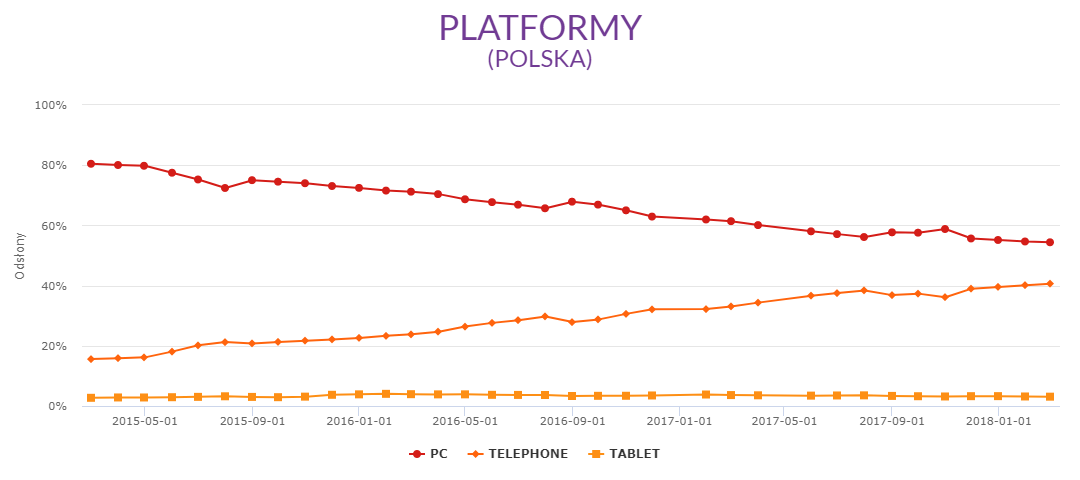
\includegraphics[width=1\textwidth]{rys/Platformy.png}
    \caption{Udział odsłon z różnych platform \newline Źródło: Gemius \cite{platformy}, 01/01/2015 - 01/03/2018r}
    \label{fig:plot1}
\end{figure}

Okazuje się, że zanotowano 20\% spadek udziału odsłon z komputera na rzecz urządzeń mobilnych. Jeżeli aktualny trend utrzyma się można prognozować, że w przyszłym roku ilo\'sć odsłon z telefonów wyrówna się z ilo\'scią odsłon z przeglądarek komputera, a w kolejnych latach procentowy udział odsłon z tego typu platform może być największy. \newline
Warto przyjrzeć w jakich rozdzielczo\'sciach ekranu są wy\'swietlane aplikacje internetowe i przeanalizować wykres \ref{fig:plot2}  
\begin{figure}[h]
    \centering
    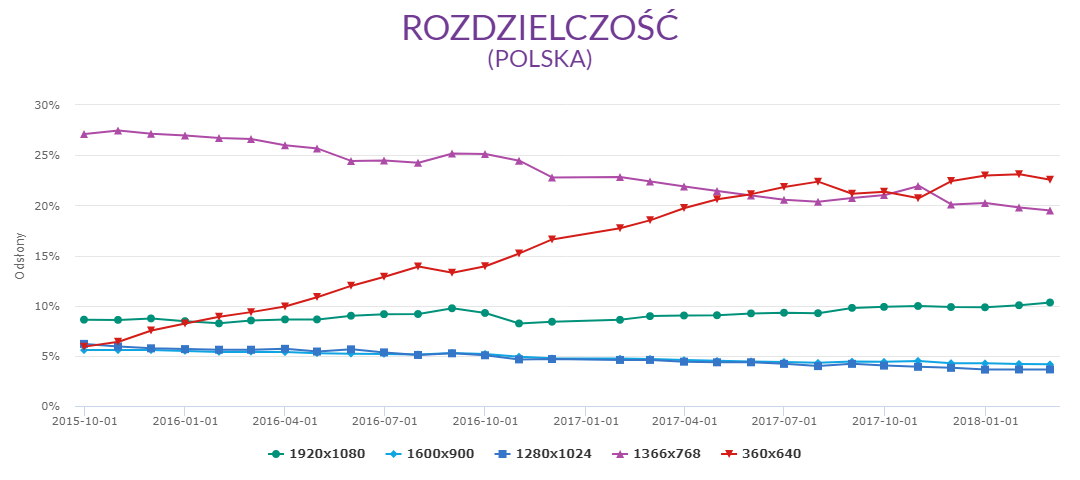
\includegraphics[width=1\textwidth]{rys/Rozdzielczosc.png}
    \caption{Udział różnych rozdzielczo\'sci  \newline Źródło: Gemius \cite{resolution}, 01/10/2015 - 01/03/2018r}
    \label{fig:plot2}
\end{figure}

Ze statystyk wynika, że aktualnie najczę\'sciej aplikacje uruchamiane są w~najmniejszej rozdzielczo\'sci (360x640). Znaczny wzrost udziału odsłon aplikacji w rozdzielczo\'sci 360x640 zaobserwowano w ciągu ostatnich kilku lat. \newline 
Zaprezentowane dane potwierdzają słuszno\'sć stosowania podej\'scia "mobile first"~przy projektowaniu interfejsu graficznego aplikacji. Zakłada on dostarczenie jak najlepszych do\'swiadczeń użytkownikowi końcowemu dla urządzeń mobilnych. Oprócz tego dane potwierdzają konieczno\'sć rozbudowy funkcjonalno\'sci aplikacji internetowych z uwzględnieniem preferencji i wymagań użytkowników korzystających z urządzeń mobilnych.

\section{Technologie dla urządzeń mobilnych}
W odpowiedzi na potrzeby użytkowników korzystających z urządzeń mobilnych powstają nowe technologie, które umożliwiają tworzenie aplikacji przyjaznych użytkownikowi. Wyróżnić można kilka podstawowych rodzajów aplikacji. W\'sród nich znajdują się te serwowane na zdalnym serwerze przez protokół HTTP/HTTPS: mobilne aplikacje sieciowe oraz progresywne aplikacje internetowe. Są one tworzone za pomocą technologii webowych, czyli języka HTML, CSS i JavaScript. Z aplikacji takich można korzystać poprzez przeglądarkę internetową dostępną na urządzeniu mobilnym. Nowym rozwiązaniem, którego celem jest jak najszybsze dostarczenie tre\'sci użytkownikowi korzystającemu z aplikacji na urządzeniu mobilnym są przyspieszone strony mobilne (ang. Accelerated Mobile Pages). Innym rodzajem są aplikacje wymagające instalacji na danej platformie. Do tej grupy zaliczają się aplikacje natywne oraz aplikacje hybrydowe. \newline Poniżej  zaprezentowano pięć kluczowych technologii stosowanych przy tworzeniu produktów na urządzenia mobilne, z uwzględnieniem ich wad i zalet.

\subsection*{Mobilne aplikacje webowe (ang. Mobile Web Apps)}
\noindent Aplikacje tworzone przy pomocy hipertekstowego języka znaczników HTML, kaskadowego arkusza stylów CSS oraz skryptowego języka programowania JavaScript. Aplikacja webowa pracuje na zdalnym serwerze i jest serwowana przez protokół HTTP(ang. Hypertext Transfer Protocol). Użytkownik końcowy może korzystać z aplikacji na urządzeniu mobilnym poprzez przeglądarkę internetową zainstalowaną na danym urządzeniu. Dostęp do aplikacji możliwy jest poprzez unikalny adres URL. Zaletą tej technologii jest stosunkowo krótki czas tworzenia, brak konieczno\'sci instalacji i uniwersalno\'sć - raz napisana aplikacja działa na różnych platformach i urządzeniach. Wymaga przeglądarki i dostępu do sieci. Wadą tego typu technologii jest brak możliwo\'sci pracy w trybie Offline oraz brak dostępu do funkcjonalno\'sci typowych dla urządzeń mobilnych (np. geolokalizacji, kamery, powiadomień).

\subsection*{Aplikacje natywne (ang. Native Apps)}
\noindent Aplikacje przeznaczone dla konkretnej platformy mobilnej (np. Android~lub~iOS). Wymagają stosowania przez deweloperów odpowiednich języków programowania oraz narzędzi deweloperskich (np. Eclipse i Java dla platformy Android, Xcode i język C dla iOS). Biorąc pod uwagę do\'swiadczenia użytkownika końcowego korzystającego z urządzenia mobilnego, tego typu aplikacje wyglądają i działają najlepiej. Zaletą tej technologii jest możliwo\'sć pracy w trybie Offline, działanie w trybie pełnoekranowym, możliwo\'sć korzystania z funkcjonalno\'sci urządzeń mobilnych (takich jak kamera, geolokalizacja, bluetooth), natychmiastowy czas ładowania pierwszego ekranu, szybki dostęp z poziomu ekranu głównego. Niekorzystny z perspektywy użytkownika jest proces instalacji aplikacji, który często wymaga kilku kroków i zajmuje dużo czasu. Proces tworzenia aplikacji natywnych jest bardziej skomplikowany niż w przypadku aplikacji webowych. Wymaga od programisty do\'swiadczenia i znajomo\'sci konkretnej technologii. W przypadku chęci uzyskania produktu wieloplatformowego konieczne jest tworzenie kilku aplikacji.

\subsection*{Progresywne aplikacje internetowe (ang. Progressive Web Apps)}
\noindent Szczególny rodzaj mobilnych aplikacji webowych, który powstał w 2015 roku. Rozwiązanie to polega na progresywnym rozszerzeniu aplikacji sieciowej, w~taki sposób, aby wyglądała i działała jak aplikacja natywna. Progresywne aplikacje webowe łączą w sobie najlepsze cechy aplikacji natywnych z najlepszymi cechami aplikacji sieciowych. Dzięki temu powstaje aplikacja, która nie~wymaga instalacji. Uruchamiana jest dzięki przeglądarce zainstalowanej~na urządzeniu mobilnym. Aplikacja taka jest szybka, niezawodna (działa w~trybie offline lub przy niestabilnym połączeniu sieciowym) i angażująca użytkownika \cite{pwa}. Zaangażowanie to uzyskuje się dzięki możliwo\'sci przypięcia ikony aplikacji do ekranu głównego urządzenia mobilnego i szybkiej możliwo\'sci uruchomienia oraz dzięki możliwo\'sci wykorzystania powiadomień typu push, co~nie jest typową funkcjonalno\'scią aplikacji sieciowych. Ten rodzaj technologii pozwala na tworzenie produktów bezpiecznych (ze zwględu na~serwowanie przez protokół HTTPS) oraz przyjaznych użytkownikowi. Ponadto możliwe jest wykorzystanie funkcjonalno\'sci typowych dla urządzeń mobilnych (np.~kamera, mikrofon, kalendarz, bluetooth). Problemem w tego typu aplikacjach jest wsparcie przeglądarek internetowych. Tylko nowoczesne przeglądarki umożliwiają korzystanie z pełnej funkcjonalno\'sci progresywnych aplikacji internetowych. Szczegółowy opis technologii umieszczono~w~rozdziale "\nameref{chap:pwa}".

\subsection*{Aplikacje hybrydowe (ang. Hybrid Apps)}
\noindent Idea aplikacji hybrydowych polega na wykorzystaniu najlepszych cech aplikacji natywnych i aplikacji webowych Do stworzenia aplikacji wykorzystuje się języki typowe dla aplikacji webowych (HTML, JavaScript, CSS). Kod źródłowy aplikacji hybrydowej jest pakowany do specjalnego kontenera Widoku Sieciowego (WebView) \cite{hybrid}. Takie rozwiązanie umożliwia tworzenie aplikacji, które wyglądają jak aplikacje natywne i są wieloplatformowe. Produkty tego typu wymagają instalacji i są dystrybuowane przez sklepy producentów systemów operacyjnych. Aplikacje hybrydowe działają w trybie online i offline. Są bezpiecznym rozwiązaniem i umożliwiają korzystanie z funkcjonalno\'sci urządzeń mobilnych dzięki zastosowaniu pluginów i odpowiednich narzędzi. Ten rodzaj technologii bardzo się rozwija w ostatnim czasie. Ciągle powstają nowe narzędzia i frameworki pozwalające na tworzenie wieloplatformowych aplikacji za pomocą technologii webowych. Szczegółowy opis aplikacji hybrydowych zawarty jest w rozdziale "\nameref{chap:hybrid}".

\subsection*{Przyspieszone strony mobilne (ang. Accelerated Mobile Pages)}
\noindent Technologia Accelerated Mobile Pages powstała w wyniku współpracy firmy Google z wydawcami na całym \'swiecie w ramach projektu Digital News Initiative. Główna idea tego rozwiązania to maksymalna optymalizacja czasu renderowania elementów znajdujących się na stronie internetowej oraz redukcja ładowania dodatkowych bibliotek do minimum \cite{amp}. W celu realizacji tych założeń powstała biblioteka typy open-source - AMP. Służy ona do tworzenia stron internetowych, które szybko się ładują i są atrkacyjne dla użytkowników końcowych \cite{amp2}. Przy tworzeniu tego typu stron korzysta się z języków programowania typowych dla aplikacji webowych (HTML, JavaScript, CSS). W przypadku tego rozwiązania nie ma problemu z kompatybilno\'scią przeglądarek i platform, na których strony AMP są używane. Ten rodzaj technologii nie daje możliwo\'sci korzystania z funkcjonalno\'sci typowych dla urządzeń mobilnych jak kamera, bluetooth czy kalendarz.

%Instant apps??


%-----------------
% Progresywne aplikacje internetowe
%-----------------
\chapter{Progresywne aplikacje internetowe} \label{chap:pwa}
\noindent Twórcą technologii jest firma Google. Progresywne aplikacje internetowe powstały w odpowiedzi na ograniczenia standardowych aplikacji webowych względem urządzeń mobilnych. PWA (ang Progressive Web Apps) tworzone są za pomocą hipertekstowego języka znaczników HTML, kaskadowego arkusza stylów CSS oraz skryptowego języka programowania JavaScript. Idea tego rozwiązania polega na rozszerzeniu podstawowej funkcjonalno\'sci aplikacji internetowych w sposób progresywny, aby w trakcie korzystania z PWA do\'swiadczenia użytkownika były podobne, jak przy korzystaniu z klasycznej aplikacji natywnej.
\subsection*{Cechy Progresywnych Aplikacji Internetowych}
\begin{itemize}
\item{\textbf{niezawodno\'sć i niezależno\'sć od sieci} - aplikacja ma dostarczać tre\'sci użytkownikowi w sposób niezawodny, bez względu na stan sieci (również w stanie Offline). Realizacja tej cechy jest możliwa dzięki zastosowaniu mechanizmu Service Worker w połączeniu z interfejsem API magazynu do przechowywania danych po stronie klienta przeglądarki np. Cache Storage API lub IndexedDB. Szczegółowy opis mechanizmu umieszczono w podrozdziale "\nameref{subs:sw}",}
\item{\textbf{szybko\'sć działania} - odpowiedzi serwera na interakcje użytkownika powinny być natychmiastowe, animacje podczas przewijania powinny działać w sposób płynny. W celu optymalizacji wydajno\'sci wykorzystuje się ponowne wykorzystanie pobranych zasobów (buforowanie).Ma to wpływ róznież ze względów ekonomicznych. Minimalizacja kolejnych cykli wymiany danych nie blokuje przeglądarki i nie przyczynia się do większych kosztów transferu,}
\item{\textbf{możliwo\'sć angażowania użytkownika} - aplikacje typu PWA mogą zwiększać zaangażowanie użytkowników dzięki zastosowaniu notyfikacji typu push oraz możliwo\'sci przypięcia ikony aplikacji do ekranu głównego urządzenia mobilnego. Opcja ta jest możliwa dzięki standardowi Web App Manifest. Szczegółowy opis standardu znajduje się w podrozdziale "\nameref{subs:manifest}",}
\item{\textbf{bezpieczeństwo} - wymagane jest bezpieczne połączenie, aplikacja musi być serwowana przez protokół HTTPS,}
\item{\textbf{integrowalne} - istnieje możliwo\'sć integracji z innymi aplikacjami oraz urządzeniami smartphone'a poprzez zewnętrzne API,}
\item{\textbf{responsywno\'sć} - aplikacja dobrze wygląda bez względu na urządzenie i ekran, z którego korzysta użytkownik,}
\item{\textbf{progresywno\'sć} - aplikacja działa niezależnie od użytkownika i przeglądarki, z której on korzysta,}
\item{\textbf{wykrywalno\'sć} - wykrywanie aplikacji poprzez silniki przeglądarek jest możliwe dzięki standardom W3C: manifest W3C \cite{manifest} oraz Service Worker W3C \cite{service},}
\item{\textbf{uniwersalno\'sć} - aplikacja działa poprawnie na różnych platformach,}
\item{\textbf{dostępno\'sć} - progresywne aplikacje internetowe są zarówno instalowalne (istnieje możliwo\'sć przypięcia ikony aplikacji do ekranu głównego z opcją szybkiego uruchomienia) jak i linkowalne tzn. do aplikacji można dostać się przez przeglądarkę za pomocą unikalnego adresu URL, dzięki temu udostępnianie tre\'sci jest łatwe,}
\item{\textbf{aktualno\'sć danych} - dzięki funkcjonalno\'sciom Service Workera możliwe jest od\'swieżanie danych, dzięki czemu dane aplikacji są aktualne.}

\end{itemize}
podlinkuj
https://developers.google.com/web/updates/2015/12/getting-started-pwa
\newpage

%wymagania
\section{Wymagania stawiane progresywnym aplikacjom sieciowym}
Progresywne aplikacje webowe są serwowane na zdalnym serwerze. Dostęp do nich możliwy jest tak jak w przypadku klasycznych aplikacji sieciowych przez przeglądarkę. Z technicznego punktu widzenia zwykła aplikacja webowa jest nazywana progresywną, gdy spełnione są następujące warunki \cite{ieee}:
\begin{itemize}
\item{aplikacja serwowana jest poprzez protokół HTTPS (ang. Hypertext Transfer Protocol Secure), co zapewnia użytkownikowi bezpieczne korzystanie z aplikacji,}
\item{aplikacja korzysta z minimum jednego mechanizmu Service Worker,}
\item{aplikacja wykorzystuje Web App Manifest, który zawiera metadane dotyczące nazwy aplikacji, ikon, startowego adresu URL, itp.}
\end{itemize}
%file:///C:/mgr/sources/Accessing%20the%20impact%20of%20service%20workers%20on%20the%20energy%20efficiency%20of%20Progressive%20Web%20Apps.pdf

%architektura powłoki pwa
\section{Architektura powłoki aplikacji progresywnych}
\noindent Powłoka systemowa aplikacji tworzy interfejs użytkownika i generowana jest za pomocą kodu HTML, CSS, JavaScript. Jest to minimalny zestaw plików niezbędny do załadowania strony głównej aplikacji. W przypadku zwykłej aplikacji sieciowej przy każdym wej\'sciu na stronę pobierane są wszystkie pliki (tre\'sci dynamiczne jak i statyczne). Wiąże się to z pewnym czasem oczekiwania użytkownika na załadowanie aplikacji. Istnieją pliki, które są wykorzystywane wielokrotnie. Progresywne aplikacje internetowe umożliwiają przechowywanie takich plików w pamięci podręcznej przeglądarki (cache). Dzięki temu możliwa jest minimalizacja czasu oczekiwania użytkownika aplikacji na załadowanie strony. \\
Powłokę systemową aplikacji progresywnych można porównać do pakietu kodu aplikacji natywnej publikowanego w sklepie. Powłoka systemowa odpowiada za niezawodno\'sć i wydajno\'sć. Dzięki niej interfejs użytkownika zapisuje się lokalnie, a tre\'sć pobierana jest dynamicznie przez interfejs API. Wymagania stawiane powłoce systemowej to przede wszystkim szybko\'sć wczytywania, dynamiczne wy\'swietlanie tre\'sci, możliwo\'sć zapisania w pamięci podręcznej.\\
 Architektura powłoki systemowej aplikacji to po\'srednik między infrastrukturą aplikacji i interfejsem, a danymi.  Dzięki mechanizmowi Service Worker możliwe jest zapisanie lokalne w pamięci podręcznej infrastruktury i interfejsu.  \newline

%korzysci
\subsection*{Korzy\'sci wynikające z modelu powłoki}
\noindent Zastosowanie architektury powłoki niesie ze sobą wiele korzy\'sci dla użytkowników aplikacji. W\'sród nich można wymienić:
\begin{itemize}
\item{Niezawodna wydajno\'sć i szybko\'sć działania aplikacji.\\ Powtórne otwieranie strony jest bardzo szybkie. Tre\'sci statyczne oraz elementy tworzące interfejs użytkownika (np. HTML, CSS, JavaScript, obrazy) są zapisywane w pamięci podręcznej przeglądarki (pamięci cache). Wykonuje się to przy pierwszym uruchomieniu aplikacji w danej przeglądarce. Tre\'sć może trafić do pamięci podręcznej przeglądarki przy pierwszym uruchomieniu aplikacji, ale jest ładowana w momencie, w którym jest potrzebna do prawidłowego działania aplikacji (okre\'slona przez programistę w kodzie źródłowym aplikacji),}
\item{Interakcje jak w aplikacjach natywnych.}\\ Użytkownicy, którzy korzystają z aplikacji sieciowych z architekturą powłoki mają do\'swiadczenia (ang. user experience) podobne jak przy korzystaniu z aplikacji natywnej. Czas interakcji na akcję użytkownika jest bardzo krótki. Nawigacja jest podobna do nawigacji w aplikacjach natywnych. Aplikacje progresywne działają w trybie Offlie, co jest nietypowe dla aplikacji sieciowych.
\item{Ekonomiczne użycie danych. \\Podej\'scie zakładające minimalne użycie danych i rozsądne zapisywanie danych do pamięci podręcznej. Zapisywanie zbyt dużej ilo\'sci mało istotnych danych (np. obrazów w dużym rozmiarze, które są wy\'swietlane tylko na jednej stronie) powoduje pobieraniem zbyt dużej ilo\'sci danych, niż jest to potrzebne. Wpływa to na koszt połączenia i danych. }
\end{itemize}

%wymagania architektury powłoki
\subsection*{Wymagania stawiane architekturze powłoki aplikacji}
 Powłoka aplikacji powinna \cite{shell}:
\begin{itemize}
\item{szybko się ładować,}
\item{używać jak najmniejszej ilo\'sci danych,}
\item{używać zasobów statycznych z pamięci podręcznej,}
\item{oddzielać tre\'sci od nawigacji,}
\item{pobierać i wy\'swietlać tre\'sci specyficzne dla strony(HTML, JSON, itp.),}
\item{dynamicznie wy\'swietlać tre\'sci}
\end{itemize}
https://blog.ionicframework.com/what-is-a-progressive-web-app/ App Shell
https://google-developer-training.gitbooks.io/progressive-web-apps-ilt-concepts/content/docs/introduction-to-progressive-web-app-architectures.html
\subsection*{Wzorce architektoniczne PWA}
%https://google-developer-training.gitbooks.io/progressive-web-apps-ilt-concepts/content/docs/introduction-to-progressive-web-app-architectures.html#patterns
PWA Architectural Patterns
\section{Standardy progresywnych aplikacji webowych}
\subsection{Service Worker} \label{subs:sw}
Service Worker jest rodzajem Web Worker'a, który jest uruchamiany razem z całą aplikacją sieciową, ale jego czas życia zależy od realizacji zdarzeń, które są przypisane w aplikacji. Mechanizm zawiera sieć proxy 
https://w3c.github.io/ServiceWorker/
Some of its services include a network proxy written in JavaScript that intercepts HTTP requests made from web pages (including HTTPS). For example, a service worker can intercept outgoing network requests and provide alternatives when the network is offline (such as by serving up cached web content). Service workers can also respond to incoming events, such as push notifications.
Service workers depend on two APIs to work effectively: Fetch (a standard way to retrieve content from the network) and Cache (a persistent content storage for application data. This cache is persistent and independent from the browser cache or network status.)
%Using Libraries to Code Service Workers z https://google-developer-training.gitbooks.io/progressive-web-apps-ilt-concepts/content/docs/introduction-to-progressive-web-app-architectures.html#patterns

edge cases of service workers:
https://www.youtube.com/watch?v=zuGE3eFQD9I 16:20

\subsection{Web App Manifest} \label{subs:manifest}
web app manifest W3C Spec https://w3c.github.io/manifest/

A JSON-formatted file named manifest.json that is a centralized place to put metadata that controls how the web application appears to the user and how it can be launched. (Do not confuse this with amanifestfile used by AppCache.) PWAs use the web app manifest to enable "add to homescreen".
\section{Praca w trybie Offline}
%ważne tabelka z limitami pamięci cache:
http://grinninggecko.com/2011/02/24/developing-cross-platform-html5-offline-app-1/
%https://developer.mozilla.org/en-US/docs/Web/API/IndexedDB_API/Browser_storage_limits_and_eviction_criteria
%storage - przechowywanie danych w przegladarce - porównanie różnych sposobów (Web Storage, Web SQL Database, Indexed Database (IndexedDB), FileSystem
https://www.html5rocks.com/en/tutorials/offline/storage/

\section{Powiadomienia}
Push push push
\section{Ograniczenia}
cache'owanie - limity
https://cloudfour.com/thinks/ios-doesnt-support-progressive-web-apps-so-what/
\section{Narzędzia deweloperskie}



PWA Tooling GOals & Philosophy:
https://www.youtube.com/watch?v=zuGE3eFQD9I
https://google-developer-training.gitbooks.io/progressive-web-apps-ilt-concepts/content/docs/lighthouse-pwa-analysis-tool.html

SPecific Tools
https://www.youtube.com/watch?v=zuGE3eFQD9I: 
React, 
\subsection*{Lighthouse}
\subsection*{Zakładka Applications}

%-----------------
% Aplikacje hybrydowe
%-----------------
\chapter{Aplikacje hybrydowe} \label{chap:hybrid}
\section{Porównanie natywnych aplikacji i hybrydowych}
\section{Przegląd narzędzi}
\section{Wady i zalety}

%-----------------
% Implementacja aplikacji
%-----------------
\chapter{Implementacja aplikacji}/

%-----------------
% Porównanie PWA i HA
%-----------------
\chapter{Porównanie progresywnej aplikacji internetowej i aplikacji hybrydowej}

Software Function, Source Lines of Code, and Development Effort Prediction: A Software Science Validation:
https://ieeexplore.ieee.org/abstract/document/1703110/references

 A. J. Albrecht, "Measuring application development productivity", Proc. IBM Applications Develop. Symp., pp. 83, 1979-Oct.-14-17.

M. H. Halstead, Elements of Software Science, New York:Elsevier, 1977.
   
 J. E. Gaffney, "Software metrics: A key to improved software development management", Conf. Comput. Sci. Statist. 13th Symp. on Interface, 1981-Mar.
 

%fajna tabelka natywne vs progresywne
%https://codeburst.io/all-you-need-to-know-about-progressive-web-app-4ba73368da66
%-----------------
% Wnioski 
%-----------------
\chapter{Wnioski}


\begin{thebibliography}{99}
\addcontentsline{toc}{chapter}{Bibliografia}
\bibitem{platformy}{http://ranking.gemius.com/pl/ranking/platforms/}
\bibitem{resolution}{http://ranking.gemius.com/pl/ranking/resolutions/}
\bibitem{pwa}{https://developers.google.com/web/progressive-web-apps/}
\bibitem{hybrid}{https://blog.strefakursow.pl/co-musisz-wiedziec-zanim-zaczniesz-tworzyc-aplikacje-mobilne/} 
\bibitem{amp}{http://antyweb.pl/strony-mobilne-jeszcze-nigdy-nie-wczytywaly-sie-tak-szybko-google-przedstawia-projekt-accelerated-mobile-pages/}
\bibitem{amp2}{https://www.ampproject.org/ru/learn/overview/}
\bibitem{shell}{http://webagility.com/posts/how-progressive-web-apps-make-the-web-great-again}
\bibitem{manifest}{https://w3c.github.io/manifest/}
\bibitem{service}{https://w3c.github.io/ServiceWorker/}
%\bibitem{ieee}{Assessing the Impact of Service Workers on the Energy Efficiency of Progressive Web Apps/}

\end{thebibliography}

\zakonczenie  % wklejenie recenzji i opinii

\end{document}
%+++ END +++
